\lecture{5}{10. Februar 2025}{Diffusion in solids}
Before talking about diffusion it is important to have a few general definitions.

\section{Diffusion}

\begin{definition}[Diffusion]
  Diffusion is the process of transporting mass by atomic motion.
\end{definition}

\begin{definition}[Diffusion mechanisms]
  The main diffusion mechanism for liquids and gasses is \textit{random} Brownian motion, whereas the main diffusion mechanism for solids is vacancy and interstitual diffusion.
\end{definition}

\begin{definition}[Interdiffusion]
  Diffusion of atoms of one material into another material.
\end{definition}

\begin{definition}[Self-diffusion]
  Atomic migration in a pure metal.
\end{definition}

\subsection{Mechanisms of diffusion}
Atoms tend to migrate from regions of high concentration to regions of low concentration. This is shown in \textbf{\autoref{fig:f5_1}}.
\begin{figure} [ht]
  \centering
  \caption{Diffusion between materials at the interface of the materials}
  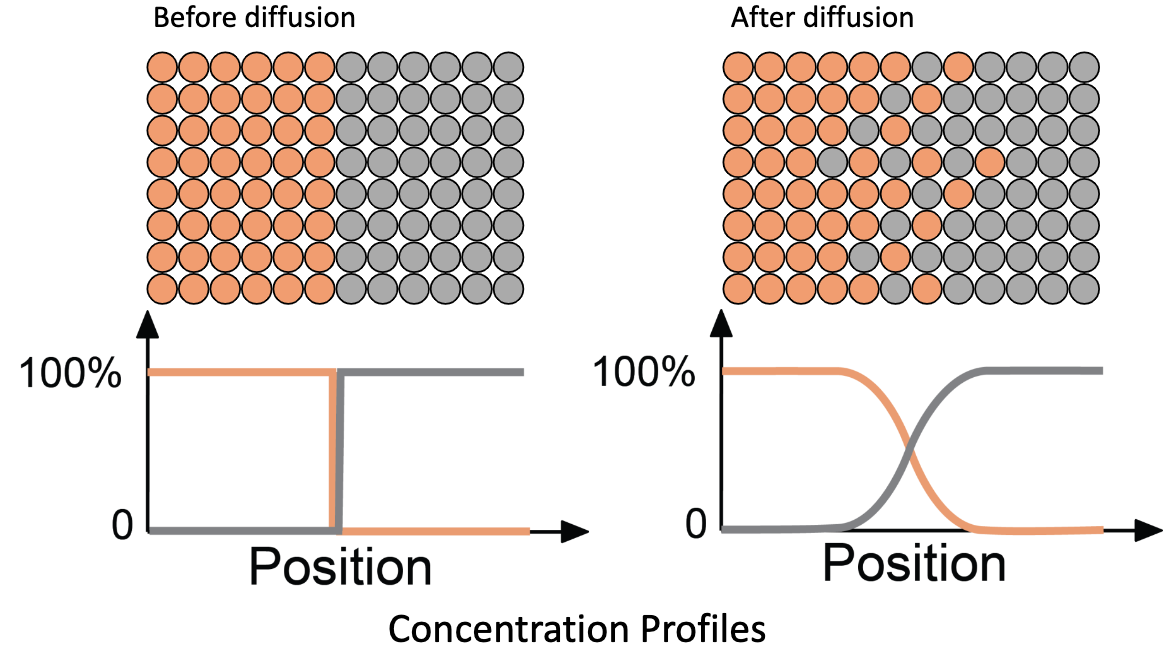
\includegraphics[width=0.5\linewidth]{./figures/f5_1.png}
  \label{fig:f5_1}
\end{figure}

It is however not only different materials that diffuse into eachother. If one labels a few different atoms in the crystal lattice of a solid, then at some later point these atoms will be in new positions due to self-diffusion. This is shown on \textbf{\autoref{fig:f5_2}}.
\begin{figure} [ht]
  \centering
  \caption{Self-diffusion in a crystal lattice}
  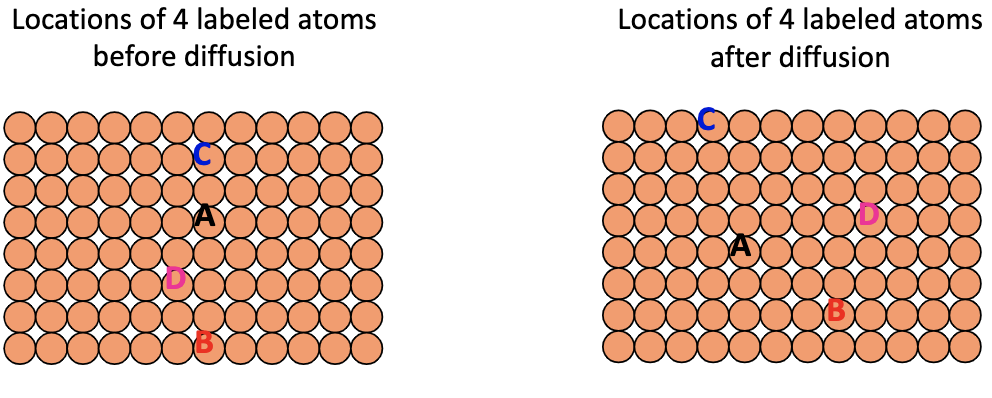
\includegraphics[width=0.5\linewidth]{./figures/f5_2.png}
  \label{fig:f5_2}
\end{figure}

\subsubsection{Vacancy diffusion}
Atoms and vacancies are always exchanging positions. This applies to both the host atoms of a lattice and the substitutional impurity atoms. In short the diffusion rate depends on the number of vacancies and the activation energy to exchange. This is the most energy-expensive form of diffusion. This process is shown in \textbf{\autoref{fig:f5_3}}.
\begin{figure} [ht]
  \centering
  \caption{Vacancy diffusion in a crystal lattice}
  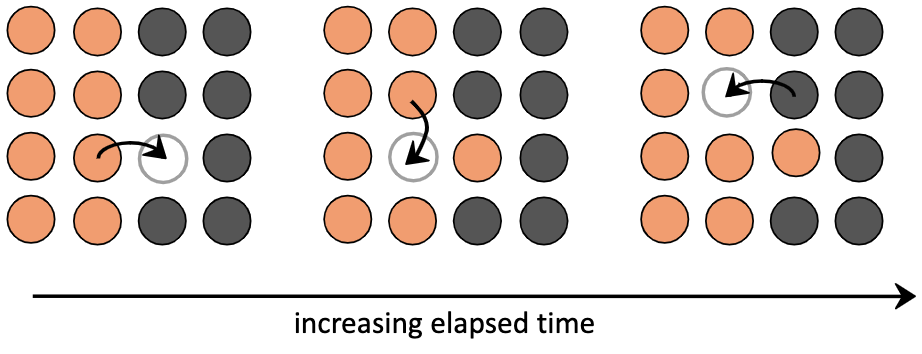
\includegraphics[width=0.5\linewidth]{./figures/f5_3.png}
  \label{fig:f5_3}
\end{figure}

\subsubsection{Interstitial diffusion}
Through the process of interstitial diffusion, (relatively) small (often C or H) atoms are able to move from one interstitial position to another. This process requires less energy and happens much more rapidly than vacancy diffusion. This process is shown in \textbf{\autoref{fig:f5_4}}.
\begin{figure} [ht]
  \centering
  \caption{Interstitial diffusion in a crystal lattice}
  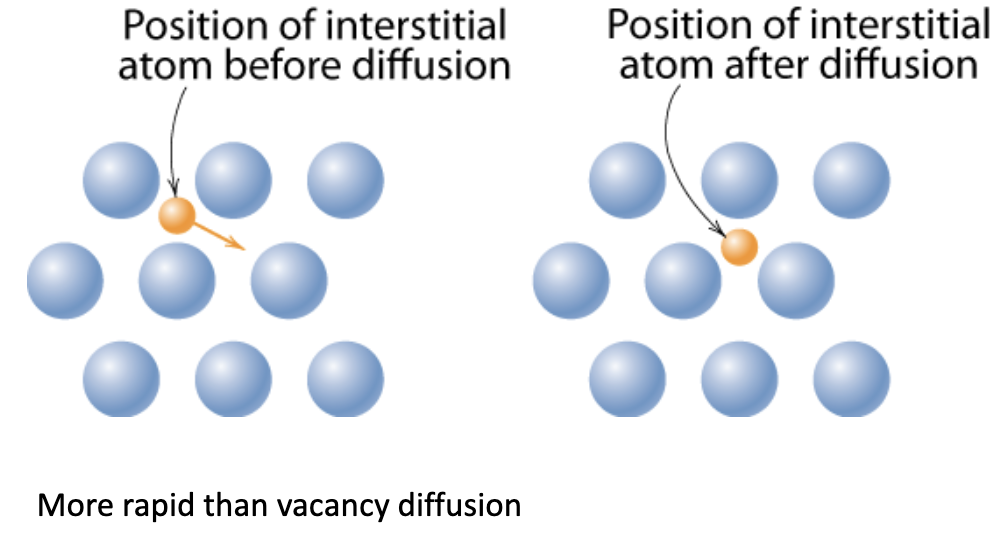
\includegraphics[width=0.5\linewidth]{./figures/f5_4.png}
  \label{fig:f5_4}
\end{figure}

\subsection{Diffusion rate}
Diffusion is a time-dependent process. The rate of diffusion is expressed as the diffusion flux, $J$.
\[
J = \mathrm{flux} = \frac{\text{mass of diffused species}}{(\mathrm{area})(\mathrm{time})} = \frac{M}{At} \left[ \unit{\frac{kg}{m^2 s}} \right] = \frac{I}{A} \frac{\mathrm{d}M}{\mathrm{d}t}
.\]
This is typically measured experimentally by finding a thin sheet (membrane) with cross-sectional area $A$. Then one imposes a concentration gradient across the membrane and measures the mass of the diffusion species $MM$ that passes through the sheet over a time period $t$. 

\subsection{Steady-state diffusion and Fick's 1st law}
Steady state diffusion (or flux) is any diffusion (or flux) that is independent of time. The flux ($J$) will then be proportional to the concentration gradient, as
\[ 
J \propto = \frac{\mathrm{d}C}{\mathrm{d}x} 
\]
where $C$ is the concentration and $x$ is the diffusion direction. Fick's first law of diffusion states that
\[ 
J = - D \frac{\mathrm{d}C}{\mathrm{d}x} 
\]
where $D$ is the diffusion coefficient. If the concentration gradient is linear then
\[ 
\frac{\mathrm{d}C}{\mathrm{d}x} \approx \frac{\Delta C}{\Delta x} = \frac{C_2 - C_1}{x_2 - x_1} 
\]
this is also shown in \textbf{\autoref{fig:f5_5}}.
\begin{figure} [ht]
  \centering
  \caption{Linear concentration gradient}
  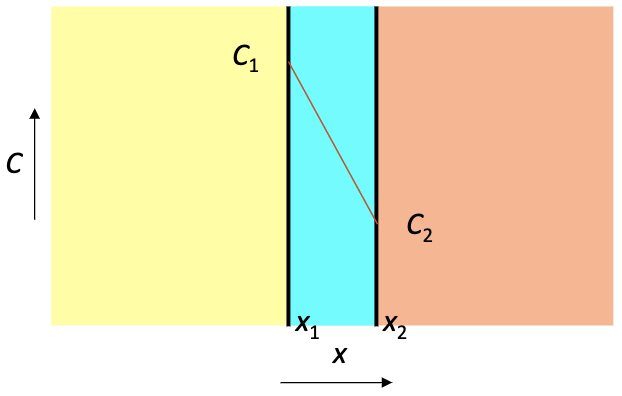
\includegraphics[width=0.5\linewidth]{./figures/f5_5.png}
  \label{fig:f5_5}
\end{figure}

\begin{exa}[Chemical protective clothing (CPC)]
  Methylene chloride is a common ingredient of paint removers. Besides being an irritant, it also may be absorbed through the skin. When using this paint remover, protective gloves should be worn.

  We want to investigate whether butyl rubber gloves (\qty{0,04}{cm} thick) commonly found in the kitchen can be used as protective gloves. It should be noted that the maximum allowable flux for a \qty{150}{lbs} person is less than \qty{3,5e-7}{\g.\cm^{-2}.\s^{-1}}. Our goal is thus to calculate the diffusion flux of methylene chloride through the gloves. We have that
  \[ 
  J = -D \frac{\mathrm{d}C}{\mathrm{d}x} = -D \frac{C_2 - C_1}{x_2 - x_1}
  .\]
  We know that
  \begin{align*}
    D  &= \qty{110e-8}{\frac{cm^2}{s}} \\
    C_1 &= \qty{0,44}{\frac{g}{cm^3}}  \\
    C_2 &= \qty{0,02}{\frac{g}{cm^3}} \\
    x_1 - x_2 &= \qty{0,04}{cm} 
  .\end{align*}
  We thus have
  \[ 
  J = -\qty{110e-8}{\frac{cm^2}{s}} \cdot \frac{\qty{0,02}{\frac{g}{cm^3}} - \qty{0,44}{\frac{g}{cm^3}}}{\qty{0,04}{cm}} = \qty{1.16e-5}{\frac{g}{cm^2}}
  .\]
  We thus have that $J = \qty{1,16e-5}{\frac{g}{cm^2}} > \qty{3,5e-7}{\frac{g}{cm^2 s}}$ and therefore the butyl gloves are not good enough to be able to use with the paint remover.
\end{exa}

\subsection{Effect of temperature}
The diffusion coefficient $D$ increases with increasing temperature $T$. We have that
\begin{equation} \label{eq:diff}
  D = D_0 e^{- \frac{Q_d}{RT}}
\end{equation}
where $D_0 [\unit{\frac{m^2}{s}}]$ is the \textit{theoretical} diffusion coefficient at $T = \qty{0}{K}$, $Q_d [\unit{\frac{J}{mol}}]$ is the activation energy for diffusion, $R$ is the gas constant and $T [\unit{K}]$ is the absolute temperature. A general graph of this is shown in \textbf{\autoref{fig:f5_6}}, whilst some different diffusion coefficients for some common material combinations are shown on \textbf{\autoref{fig:f5_7}}. 
\begin{figure} [ht]
  \centering
  \caption{Graph of diffusion coefficient as a function of temperature}
  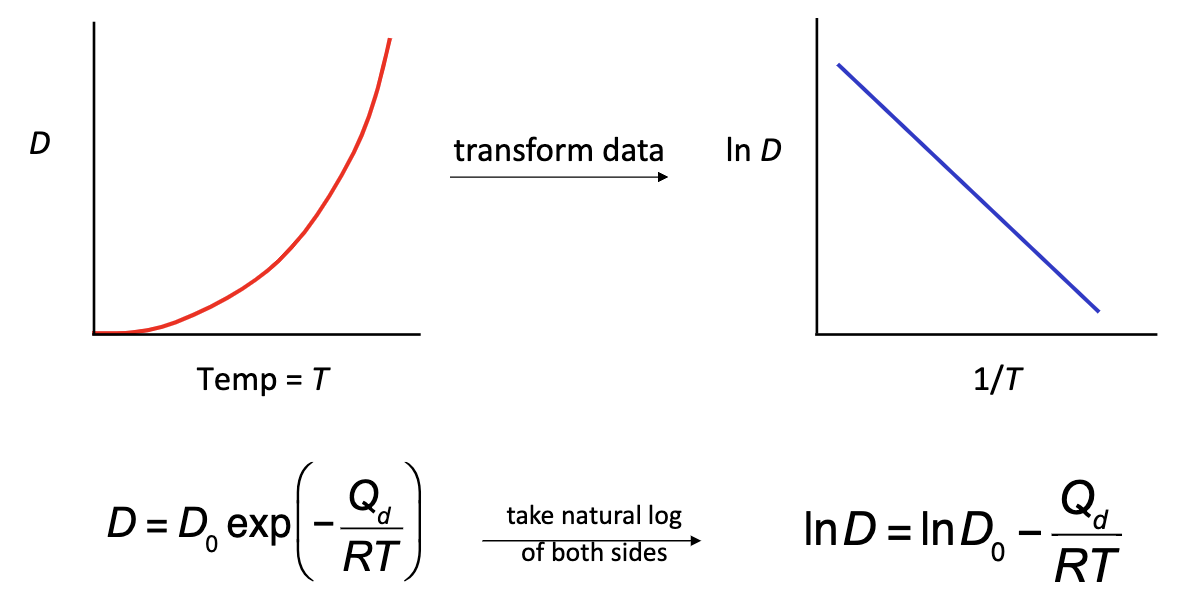
\includegraphics[width=0.6\linewidth]{./figures/f5_6.png}
  \label{fig:f5_6}
\end{figure}
\begin{figure} [ht]
  \centering
  \caption{Common material combinations and their diffusion coefficients}
  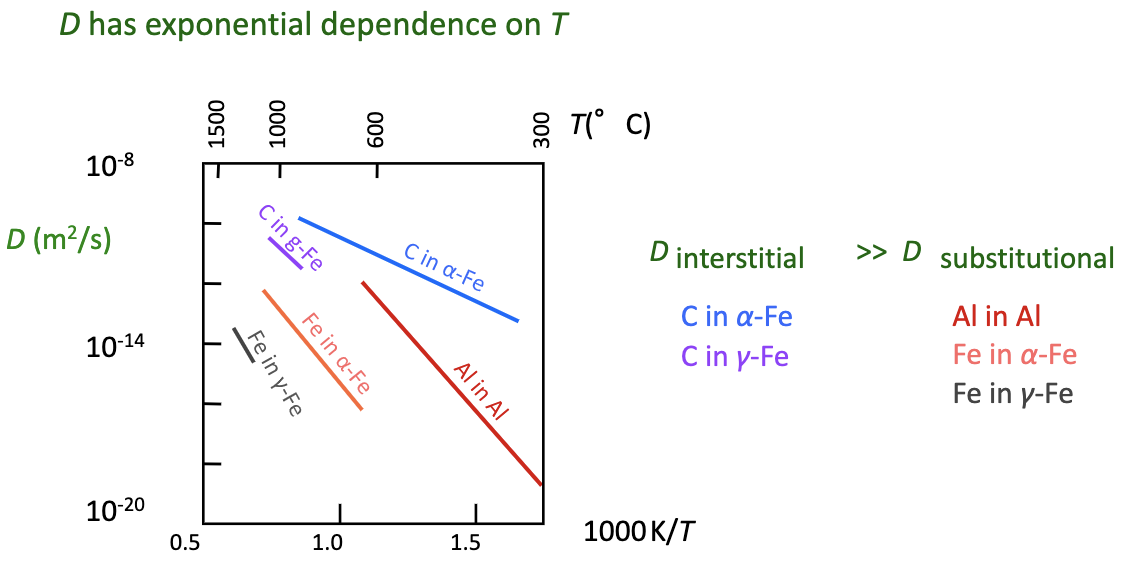
\includegraphics[width=0.7\linewidth]{./figures/f5_7.png}
  \label{fig:f5_7}
\end{figure}
A parallel to \textbf{\autoref{eq:diff}}, which would allow one to calculate the diffusion coefficient at one temperature if one knows the diffusion coefficient at another, can be found by first knowing the diffusion coefficients $D_1$ and $D_2$ at two temperatures $T_1$ and $T_2$. We then have that
\begin{align*}
  \ln D_2 &= \ln D_0 - \frac{Q_d}{R} \left( \frac{1}{T_2} \right) \\
  \ln D_1 &= \ln D_0 - \frac{Q_d}{R} \left( \frac{1}{T_1} \right)
.\end{align*}
We can now subtract the second equation above from the first as
\[ 
  \ln D_2 - \ln D_1 = \ln \frac{D_2}{D_1} = - \frac{Q_d}{R} \left( \frac{1}{T_2} - \frac{1}{T_1} \right)
.\]
And if we take the exponential on both sides we get
\[ 
  D_2 = D_1 e^{- \frac{Q_d}{R} \left( \frac{1}{T_2} - \frac{1}{T_1} \right)}
.\]

\begin{exa}[Finding the diffusion coefficient at another temperature]
  Suppose we known that the diffusion coefficient and activation energy for Cu in Si are
  \begin{align*}
    D_1(\qty{300}{\celsius}) &= \qty{7,8e-11}{\frac{m^2}{s}} \\
    Q_d(\qty{300}{\celsius}) &= \qty{41,5}{\frac{kJ}{mol}} 
  .\end{align*}
  We now want to calculate the diffusion coefficient at \qty{350}{\celsius} .
  \bigbreak
  We can use the formula for calculating the diffusion coefficient at another temperature as
  \begin{align*}
    D_2 &= D_1 e^{- \frac{Q_d}{R} \left( \frac{1}{T_2} - \frac{1}{T_1} \right)} \\
    &= \qty{7,8e-11}{\frac{m^2}{s}} e^{- \frac{\qty{41,5}{\frac{kJ}{mol}}}{R} \left( \frac{1}{\qty{623}{K}} - \frac{1}{\qty{573}{\kelvin}} \right)} \\
    &= \qty{1,569e-10}{\frac{m^2}{s}} 
  .\end{align*}
\end{exa}

\subsection{Non-steady-state diffusion and Fick's 2nd law}
For non-steady-state systems the concentration depends not only on position but also on time $C = C(x,t)$. For these kinds of systems we seek solutions to Fick's 2nd law, which can be stated as
\begin{equation} \label{eq:fick2}
  \frac{\partial C}{\partial t} = D \frac{\partial^2 C}{\partial x^2}
\end{equation}
It should be noted that this form of the equation assumes $D$ is independent of the concentration. If this is not the case the above becomes
\[ 
\frac{\partial C}{\partial t} = \frac{\partial D}{\partial x} \frac{\partial C}{\partial x} + D \frac{\partial^2 C}{\partial x^2}
\]
however in this course we will mostly (only?) be working with the first form ($D$ is independent of the concentration).

If we consider the case of copper diffusing into a bar of aluminum one might get something along the lines of \textbf{\autoref{fig:f5_8}}.
\begin{figure} [ht]
  \centering
  \caption{Copper diffusing into aluminum}
  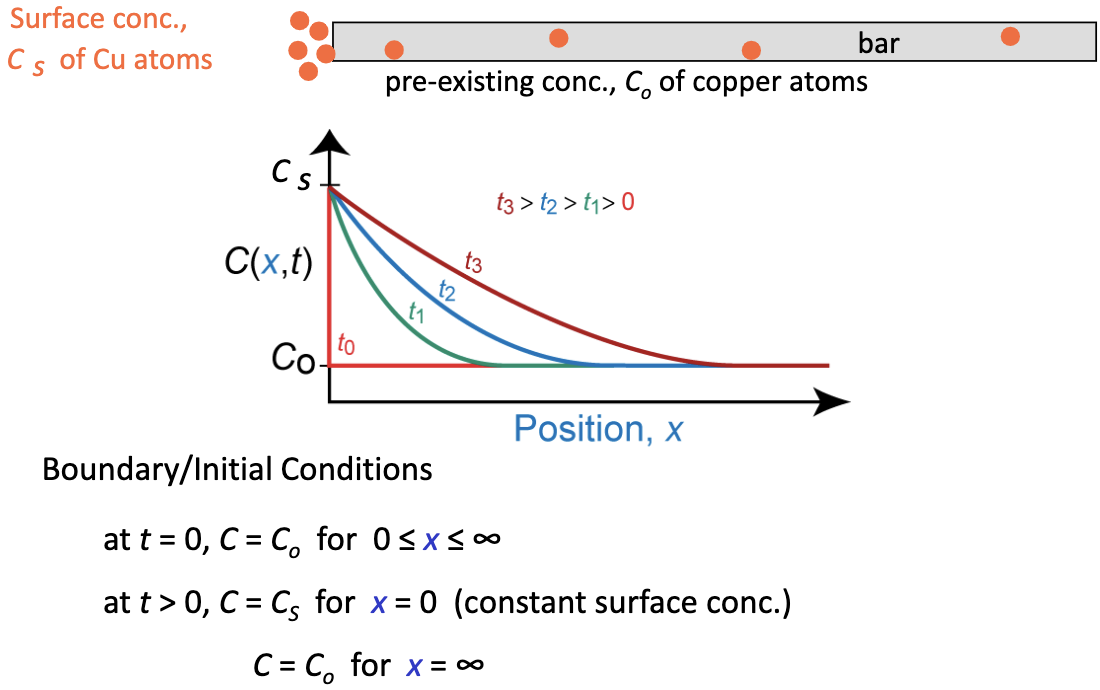
\includegraphics[width=0.75\linewidth]{./figures/f5_8.png}
  \label{fig:f5_8}
\end{figure}

The solution to \textbf{\autoref{eq:fick2}} is of the form
\[ 
\frac{C(x,t) - C_0}{C_s - C_0} = 1 - \mathrm{erf}\left( \frac{x}{2 \sqrt{D t}} \right)
\]
where $x$ is the position, $t$ is the time, $C_0$ is the bulk concentration, $C_s$ is the surface concentration, $D$ is the diffusion coefficient and $\mathrm{erf}(z) = \frac{2}{\sqrt{\pi}} \int_{0}^{z} e^{-t^2} \, \mathrm{d}t$ is the error function. 

\begin{exa}[Calculating the temperature of a diffusion process]
  An FCC iron-carbon alloy initially containing \num{0,20} wt\% C is carburized at an elevated temperature and in an atmosphere in which the surface carbon concentration is maintained at \num{1,0} wt\%. If, after \qty{49,5}{h}, the concentration of carbon is \num{0,35} wt\% at a position \qty{4,0}{mm} below the surface, determine the temperature at which the treatment was carried out.
  \bigbreak
  We start with the solution to Fick's 2nd law
  \[ 
  \frac{C(x,t) - C_0}{C_s - C_0} = 1 - \mathrm{erf} \left( \frac{x}{2 \sqrt{Dt}} \right)
  .\]
  The data needed for the problem can be found in table 5.2 of the book.
  \begin{align*}
    t &= \qty{49,5}{hr} \\
    C_x &= \num{0,35} \%  \\ 
    C_0 &= \num{0,20} \% \\
    x &= \qty{4,0e-3}{m}  \\
    C_s &= \num{1,0} \%
  .\end{align*}
  Thus we have that
  \[ 
  \frac{\num{0,35} - \num{0,2}}{1 - \num{0,2}} = 1 - \mathrm{erf}(z)
  \]
  with $z = \frac{x}{2 \sqrt{D t}}$. We thus have that
  \[ 
  \mathrm{erf}(z) = \num{0,8125}
  .\]
  We can now determine that $z = \num{0,93}$ by using the solution table to the error function found in the book. We get
  \[ 
  \num{0,93}  = \frac{x}{2 \sqrt{Dt}} \implies D = \frac{x^2}{4\num{0,93}^2 t} \implies D = \qty{2,6e-11}{\frac{m^2}{s}} 
  .\]
  We also have the formula
  \[ 
  D = D_0 e^{- \frac{Q_d}{RT}} \implies T = \frac{Q_d}{R \left( \ln D_0 - \ln D \right)}
  .\]
  From table 5.2 in the book we have that
  \begin{align*}
    D_0 &= \qty{2,3e-5}{\frac{m^2}{s}}  \\
    Q_d &= \qty{148000}{\frac{J}{mol}}
  .\end{align*}
  By plugging in the values we get that
  \[ 
  T = \qty{1300}{K} = \qty{1027}{\celsius} 
  .\]
\end{exa}
